%==============================================================================
% Sjabloon onderzoeksvoorstel bachproef
%==============================================================================
% Gebaseerd op document class `hogent-article'
% zie <https://github.com/HoGentTIN/latex-hogent-article>
% !TEX program = xelatex

% Voor een voorstel in het Engels: voeg de documentclass-optie [english] toe.
% Let op: kan enkel na toestemming van de bachelorproefcoördinator!
\documentclass{hogent-article}
\usepackage{pgfgantt}
\usepackage{pgfplots}
\pgfplotsset{compat=1.17}

% Invoegen bibliografiebestand
\addbibresource{voorstel.bib}

% Informatie over de opleiding, het vak en soort opdracht
\studyprogramme{Professionele bachelor toegepaste informatica}
\course{Bachelorproef}
\assignmenttype{Onderzoeksvoorstel}
% Voor een voorstel in het Engels, haal de volgende 3 regels uit commentaar
% \studyprogramme{Bachelor of applied information technology}
% \course{Bachelor thesis}
% \assignmenttype{Research proposal}

\academicyear{2024-2025} % TODO: pas het academiejaar aan

% TODO: Werktitel
\title{Hoe kan datareductie worden toegepast binnen AI-visionmodellen om vergelijkbare of betere performantie te bereiken zonder extra rekenkosten, en met een lager energie- en datasetverbruik?}

% TODO: Studentnaam en emailadres invullen
\author{Ayman Thomas}
\email{ayman.thomas@student.hogent.be}

% TODO: Medestudent
% Gaat het om een bachelorproef in samenwerking met een student in een andere
% opleiding? Geef dan de naam en emailadres hier
% \author{Yasmine Alaoui (naam opleiding)}
% \email{yasmine.alaoui@student.hogent.be}

% TODO: Geef de co-promotor op
\supervisor[Co-promotor]{Arshia Shariatmadar (\href{mailto:arshia@r3al.ai}{arshia@r3al.ai})}

% Binnen welke specialisatierichting uit 3TI situeert dit onderzoek zich?
% Kies uit deze lijst:
%
% - Mobile \& Enterprise development
% - AI \& Data Engineering
% - Functional \& Business Analysis
% - System \& Network Administrator
% - Mainframe Expert
% - Als het onderzoek niet past binnen een van deze domeinen specifieer je deze
%   zelf
%
\specialisation{AI & Data Engineering}
\keywords{Deep Learning, AI , INN/BNN}

\begin{document}

\begin{abstract}
De exponentiële groei van Deep Learning binnen computer vision levert modellen op met ongeziene prestaties, maar deze vooruitgang botst op harde fysieke en ecologische grenzen. Huidige trainingsmethoden vereisen enorme hoeveelheden geannoteerde data en rekenkracht, wat resulteert in hoge operationele kosten en een aanzienlijke ecologische voetafdruk. Dit onderzoeksvoorstel evalueert datareductie als noodzakelijke stap naar duurzame AI ("Groene AI"). De centrale hypothese stelt dat vision-datasets een hoge mate van redundantie bevatten en dat modellen effectief getraind kunnen worden op een strategische subset van de data zonder significant verlies aan nauwkeurigheid.

Het doel van deze studie is het valideren van een selectiemechanisme gebaseerd op onzekerheidskwantificatie. Door onderscheid te maken tussen  model onzekerheid (kennisleemtes) en data onzekerheid (ruis), kunnen de meest informatierijke datapunten geïdentificeerd worden. De methodologie omvat een kwantitatieve vergelijkende studie waarin de performantie van Convolutional Neural Networks (CNN's) op medische datasets wordt afgezet tegen varianten getraind op subsets die via onzekerheids-metrics gefilterd zijn. Hierbij wordt de impact op kritieke metrieken zoals accuratesse, trainingstijd en energieverbruik gemeten. De verwachte resultaten beogen aan te tonen dat een verschuiving van kwantiteit naar datakwaliteit leidt tot modellen die niet alleen efficiënter, maar ook breder inzetbaar zijn in resource-beperkte omgevingen.
\end{abstract}

\tableofcontents

% De hoofdtekst van het voorstel zit in een apart bestand, zodat het makkelijk
% kan opgenomen worden in de bijlagen van de bachelorproef zelf.
%---------- Inleiding ---------------------------------------------------------

% TODO: Is dit voorstel gebaseerd op een paper van Research Methods die je
% vorig jaar hebt ingediend? Heb je daarbij eventueel samengewerkt met een
% andere student?
% Zo ja, haal dan de tekst hieronder uit commentaar en pas aan.

%\paragraph{Opmerking}

% Dit voorstel is gebaseerd op het onderzoeksvoorstel dat werd geschreven in het
% kader van het vak Research Methods dat ik (vorig/dit) academiejaar heb
% uitgewerkt (met medesturent VOORNAAM NAAM als mede-auteur).
% 

\section{Inleiding}%
\label{sec:inleiding}
De afgelopen jaren hebben deep learning-\newline architecturen voor computer vision, zoals Convolutional Neural Networks (CNN’s) en Vision Transformers, een enorme sprong gemaakt in performantie. Deze modellen worden steeds vaker ingezet in diverse sectoren, variërend van industriële kwaliteitscontrole en medische beeldanalyse tot smart cities en consultancy. Deze technologische vooruitgang heeft echter een keerzijde: de huidige generatie modellen vereist enorme hoeveelheden trainingsdata en rekenkracht om tot hoge nauwkeurigheid te komen \autocite{kaplan2020scaling}. Dit resulteert niet alleen in hoge kosten voor cloud-infrastructuur en GPU-training, maar ook in een aanzienlijke ecologische voetafdruk. Daarnaast stuiten organisaties vaak op schaalbaarheidsproblemen door de tijdrovende aard van het verzamelen en annoteren van kwalitatieve data.\\

De noodzaak om deze impact te verminderen wordt ondersteund door diverse studies. Zo toont toonaangevend onderzoek van \textcite{strubell2019energy} aan dat het trainen van één enkel groot deep learning-model een CO$_2$-uitstoot kan genereren die vergelijkbaar is met de totale levensduur-emissie van vijf auto’s. Daarnaast bevestigen analyses van Google Research dat het energieverbruik van machine learning-training exponentieel toeneemt naarmate de datasetomvang en modelgrootte stijgen \autocite{patterson2021carbon}. Dit vormt een direct obstakel voor bedrijven die AI willen opschalen maar gebonden zijn aan strikte ESG-doelstellingen (Environmental, Social, and  \newline Governance).\\

\subsection{Probleemstelling}
Hoewel er technieken bestaan om AI-modellen te optimaliseren, zoals \textit{pruning}, \textit{distillation} en \newline \textit{quantization}, lossen deze het fundamentele probleem van de "datahonger" slechts gedeeltelijk op. Deze methoden verkleinen weliswaar het uiteindelijke model, maar vereisen vaak nog steeds het volledige, rekenintensieve trainingsproces op de complete dataset voordat optimalisatie kan plaatsvinden. Dit onderzoek vertrekt daarom vanuit de observatie dat er een inefficiëntie zit in de data zelf.\\

Voordat er gewerkt kan worden naar een oplossing, analyseert deze studie het probleemdomein aan de hand van de volgende kwesties: Hoe verhoudt de datasetgrootte zich nu werkelijk tot de modelperformantie in klassieke vision-mod-\newline ellen? Wat is het daadwerkelijke energie- en com\newline-pute-verbruik van een standaard trainingsproces? En cruciaal: hoeveel redundantie is er gemiddeld aanwezig in standaard vision-datasets zoals CIFAR-10 of ImageNet? De hypothese is dat veel data weinig toevoegt aan het leerproces, maar wel bijdraagt aan de ecologische last.\\

\subsection{Onderzoeksvraag en Doelstelling}
Op basis van deze problematiek luidt de centrale onderzoeksvraag van deze bachelorproef:

\begin{quote}
\textit{“Hoe kan datareductie worden toegepast binnen AI-visionmodellen om vergelijkbare of betere performantie te bereiken zonder extra rekenkosten, en met een lager energie- en datasetverbruik?”}
\end{quote}\\

Om deze vraag te beantwoorden, richt dit onderzoek zich op het oplossingsdomein door datareductie te combineren met geavanceerde onzekerheidskwantificatie. Er wordt onderzocht wat de impact is van datareductie op kritieke metrieken zoals \textit{accuracy}, F1-score en \textit{inference}-tijd. Specifiek wordt gekeken met welk percentage de dataset verminderd kan worden zonder significante daling in prestaties, en of dit leidt tot een aantoonbare verlaging van trainingstijd. De onderliggende verwachting is dat AI-visionmodellen die getraind zijn met minder, maar 'informatierijkere' data, in staat zijn om beter te generaliseren dan modellen die getraind zijn op volledige datasets vol redundantie \autocite{chen2020simple}. Het uiteindelijke doel is de weg vrijmaken voor "Groene AI", waarbij robuuste computer vision mogelijk is met lagere kosten en een minimale ecologische impact.
%---------- Stand van zaken ---------------------------------------------------

\section{Literatuurstudie}%
\label{sec:literatuurstudie}

De huidige generatie computer vision-systemen dankt haar succes aan schaalvergroting. Ontwikkelaars voeden modellen met enorme hoeveelheden data en rekenkracht om de prestaties te verhogen. Dit hoofdstuk analyseert de fysieke en ecologische grenzen van deze aanpak, de beperkingen van huidige optimalisatietechnieken en de cruciale rol van onzekerheidskwantificatie in datareductie.\\

\subsection{De grenzen van de groei: Scaling Laws} 
In de wereld van deep learning geldt vaak de aanname dat groter altijd beter is. \textcite{kaplan2020scaling} kwantificeerden dit fenomeen in hun \textit{scaling laws}. Zij toonden aan dat de foutmarge (\textit{loss}) van een model voorspelbaar daalt naarmate de hoeveelheid rekenkracht, de datasetgrootte en het aantal parameters toeneemt. Deze relatie volgt echter een machtswet (\textit{power-law}): om de prestaties lineair te verbeteren, moeten de middelen exponentieel groeien \autocite{kaplan2020scaling}. Dit maakt het trainingsproces op de lange termijn uiterst inefficiënt en onderhevig aan verminderde meeropbrengsten.\\

\subsection{Ecologische en economische impact} 
Deze inefficiëntie vormt een acuut duurzaamheidsprobleem. \textcite{strubell2019energy} toonden aan dat het trainen van één enkel groot deep learning-model een CO$_2$-uitstoot kan genereren die gelijkstaat aan de volledige levenscyclus van vijf auto’s. Recenter werk bevestigt dat het energieverbruik van AI-training exponentieel stijgt naarmate de nauwkeurigheidseisen toenemen \autocite{patterson2021carbon}. Voor bedrijven botst deze infrastructuurkost met budgettaire beperkingen en ESG-doel-\newline stellingen (Environmental, Social, and Governance). Daarnaast vormt de dataverzameling een flessenhals; het handmatig annoteren van miljoenen beelden remt de schaalbaarheid van projecten aanzienlijk.\\

\subsection{Beperkingen van huidige optimalisatietechnieken} 
De vakliteratuur zoekt naar efficiëntiewinsten, maar bestaande technieken schieten vaak tekort voor het fundamentele dataprobleem:
\begin{itemize} 
    \item \textbf{Model-centrisch:} Technieken zoals \textit{pruning} en \textit{quantization} verkleinen het model veelal \textit{na} de training. Dit versnelt de \textit{inference} op edge devices, maar vereist nog steeds de volledige dataset en rekenkracht voor het initiële, energie-intensieve trainingsproces.
    \item \textbf{Data-centrisch:} Benaderingen zoals SimCLR gebruiken \textit{contrastive learning} om robuuste representaties te leren uit ongelabelde data \autocite{chen2020simple}. Hoewel dit de afhankelijkheid van menselijke labels vermindert, blijft de noodzaak voor enorme hoeveelheden ruwe data bestaan om generalisatie te garanderen. 
\end{itemize} 
Een effectieve oplossing vereist daarom een mechanisme dat modellen in staat stelt om aan de bron selectiever te leren van een kleinere dataset.\\

\subsection{Onzekerheidskwantificatie als filter} 
Om met minder data betrouwbare beslissingen te nemen, moet een neuraal netwerk zijn eigen beperkingen kennen. Standaard vision-modellen zijn vaak \textit{overconfident}: ze geven voorspellingen met hoge zekerheid, zelfs bij foutieve resultaten. Door onzekerheid expliciet te modelleren, kan men onderscheid maken tussen slechte data en een gebrek aan kennis. De literatuur onderscheidt twee hoofdvormen, zoals gedefinieerd in de vision-context door \textcite{kendall2017uncertainties}:

\begin{enumerate} 
    \item \textbf{Data onzekerheid (Data-ruis):} Onzekerheid die inherent is aan de data zelf, zoals bewegingsonscherpte, occlusies of sensorruis. Het verzamelen van meer data lost dit type onzekerheid niet op.
    \item \textbf{Model onzekerheid (Model-\newline onwetendheid):} Onzekerheid die voortkomt uit een gebrek aan kennis in het model. Dit duidt op een tekort aan trainingsvoorbeelden in een specifiek domein en kan verholpen worden door meer relevante data toe te voegen \autocite{hullermeier2021aleatoric}. 
\end{enumerate}

Specifieke architecturen blinken uit in het vangen van deze vormen:

\subsubsection{Bayesian Neural Networks (BNN's)} 
Waar klassieke netwerken werken met vaste gewichten, beschouwt een Bayesian Neural Network gewichten als waarschijnlijkheidsverdelingen. Dit stelt BNN's in staat om \textbf{model onzekerheid} te kwantificeren. Wanneer een BNN data ziet die sterk afwijkt van de trainingsset (\textit{out-of-distribution}), neemt de spreiding in de gewichtsdistributies toe. Dit signaal identificeert waar het model kennis tekortkomt en welke data dus essentieel is voor training \autocite{blundell2015weight, jospin2022hands}.\\

\subsubsection{Interval Neural Networks (INN's)} 
In tegenstelling tot standaard netwerken die werken met exacte puntwaarden, verwerken Interval Neural Networks data als intervallen (bereiken met een onder- en bovengrens). Door gebruik te maken van interval-rekenkunde kan het netwerk direct de inherente variabiliteit en imprecisie in de input-data modelleren. Dit maakt ze uitermate geschikt voor het vangen van \textbf{data onzekerheid}: in plaats van één enkele voorspelling, genereert het model een betrouwbaarheidsinterval dat de ruis in de data omsluit \autocite{ishibuchi1993architecture}.

De combinatie van deze inzichten maakt strategische dataselectie mogelijk: door ruis (via INN-principes) en kennisleemtes (via BNN-principes) in kaart te brengen, kan een dataset gefilterd worden tot de kern die daadwerkelijk bijdraagt aan de modelperformantie.

%---------- Methodologie ------------------------------------------------------

\section{Methodologie}
\label{sec:methodologie}

In dit onderzoek wordt een kwantitatieve, experimentele benadering gehanteerd om de centrale hypothese te toetsen: is het mogelijk om met datareductie, gestuurd door onzekerheidskwantificatie, vergelijkbare modelprestaties te behalen met een lagere ecologische voetafdruk? De werkwijze is gestructureerd in vijf opeenvolgende fasen: dataset-preparatie, nulmeting (baseline), onzekerheidsanalyse, datareductie-experimenten en finale evaluatie.

Voor de validatie van de experimenten zijn drie medische datasets geselecteerd die variëren in complexiteit en omvang, om zo de generaliseerbaarheid van de methode te waarborgen. De eerste dataset, de \textbf{Brain MRI Dataset}, fungeert als binaire baseline en bevat ongeveer 3.000 MRI-scans gecategoriseerd als \textit{Tumor} of \textit{Geen Tumor}. Dit biedt een gecontroleerde omgeving om de basisprincipes van onzekerheidsfiltering te testen. Vervolgens wordt de complexiteit verhoogd met de \textbf{Chest Cancer Dataset}. Deze set bevat circa 700 afbeeldingen verdeeld over vier klassen (\textit{Adenocarcinoma}, \textit{Large Cell Carcinoma}, \textit{Squamous Cell Carcinoma} en \textit{Normal}). De beperkte omvang van deze set maakt het een ideale casus om te testen hoe goed de methode presteert in data-arme scenario's ("small data" regime). Tot slot wordt de schaalbaarheid getest op de \textbf{Alzheimer MRI Dataset}, die ongeveer 40.000 beelden omvat in vier dementie-stadia. Hier ligt de nadruk op het reduceren van redundantie in grote datasets om trainingstijden drastisch te verkorten.\\

De modelontwikkeling start met het vaststellen van een \textit{baseline}. Hiervoor wordt een standaard Convolutional Neural Network (bijvoorbeeld een ResNet-18 of EfficientNet backbone) getraind op de volledige datasets. Tijdens deze fase worden niet alleen accuratesse-metrieken (Accuracy, F1-score) vastgelegd, maar ook de computationele kosten: trainingstijd, GPU-belasting en energieverbruik (geschat via tools zoals CodeCarbon). Dit vormt het referentiepunt waartegen de "Groene AI"-modellen worden afgezet. Data-augmentatie wordt hierbij toegepast om een eerlijke vergelijking met de state-of-the-art mogelijk te maken.\\

In de kernfase van het onderzoek wordt dit basismodel uitgebreid met mechanismen voor onzekerheidskwantificatie, specifiek gericht op het onderscheid tussen epistemische en data onzekerheid (zoals beschreven in de literatuurstudie). Door gebruik te maken van technieken zoals Monte Carlo Dropout (voor BNN-benadering) of ensemb\newline-lemethoden, wordt aan elk datapunt in de trainingsset een onzekerheidsscore toegekend. Op basis van deze scores wordt de dataset iteratief gefilterd: beelden met extreem hoge model onzekerheid (zeer informatief) worden behouden, terwijl redundante beelden (lage onzekerheid) en beelden met enkel ruis (hoge data onzekerheid) systematisch worden verwijderd. \\

Vervolgens worden nieuwe modellen getraind op deze gereduceerde subsets (bijvoorbeeld 75\%, 50\% en 25\% van de originele data). De evaluatie richt zich op de trade-off tussen performantieverlies en efficiëntiewinst. Naast de standaard verwarringsmatrices wordt specifiek geanalyseerd of het model dat getraind is op de informatierijke \newline subset beter generaliseert op de testset dan een model dat getraind is op een willekeurige subset van dezelfde grootte. Dit toont aan of de onzekerheidsfilter daadwerkelijk waarde toevoegt bovenop simpele dataverwijdering. De bevindingen worden uiteindelijk vertaald naar een advies voor duurzame modeltraining.

\vspace{2em}

\noindent \textbf{Planning en Fasering} \\
Onderstaand schema visualiseert de tijdsplanning. De linkerkolom toont de officiële deliverables en deadlines, terwijl de rechterkolom de corresponderende onderzoeksactiviteiten weergeeft die nodig zijn om deze mijlpalen te behalen.

\begin{center}
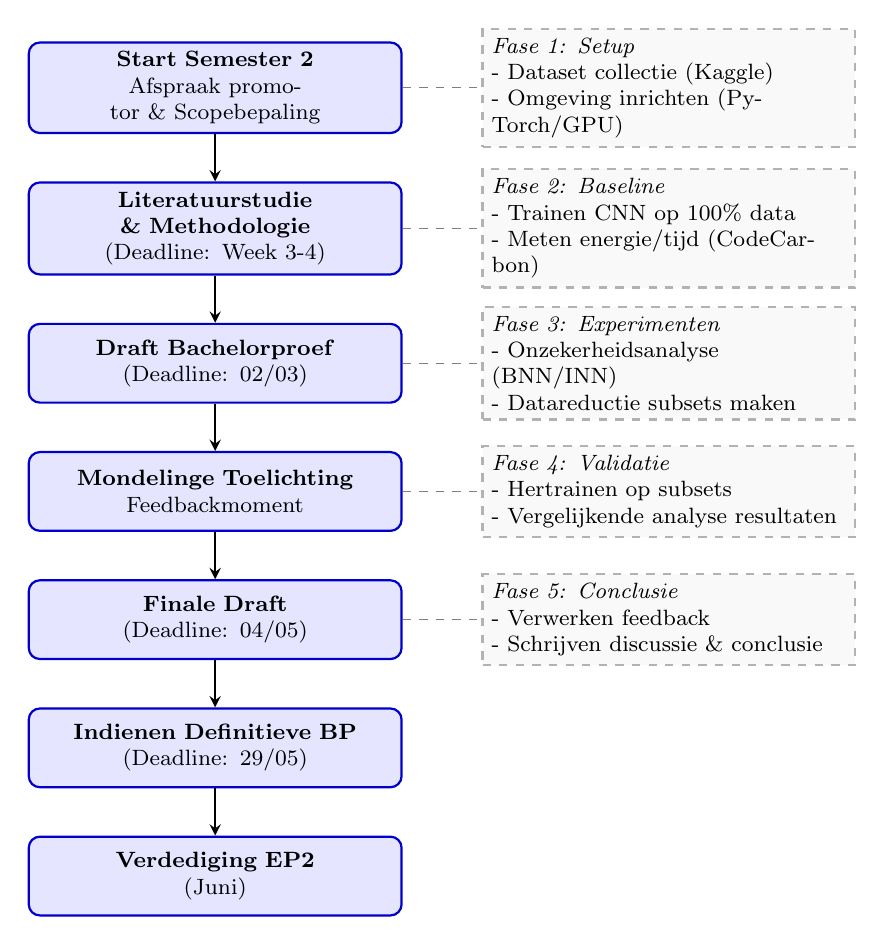
\begin{tikzpicture}[
    node distance=0.6cm and 1cm,
    every node/.style={font=\footnotesize},
    % Stijl voor deadlines/deliverables (Links)
    milestone/.style={rectangle, rounded corners, draw=blue!80!black, thick, fill=blue!10,
                      text width=4.5cm, align=center, minimum height=1cm},
    % Stijl voor onderzoeksactiviteiten (Rechts)
    task/.style={rectangle, draw=gray!60, dashed, thick, fill=gray!5,
                 text width=4.5cm, align=left, minimum height=1cm},
    arrow/.style={->, thick, >=stealth}
]

% --- Kolom 1: Deadlines ---
\node[milestone] (start) {\textbf{Start Semester 2} \\ Afspraak promotor \& Scopebepaling};
\node[milestone, below=of start] (lit) {\textbf{Literatuurstudie \& Methodologie} \\ (Deadline: Week 3-4)};
\node[milestone, below=of lit] (draft) {\textbf{Draft Bachelorproef} \\ (Deadline: 02/03)};
\node[milestone, below=of draft] (talk) {\textbf{Mondelinge Toelichting} \\ Feedbackmoment};
\node[milestone, below=of talk] (finaldraft) {\textbf{Finale Draft} \\ (Deadline: 04/05)};
\node[milestone, below=of finaldraft] (bp) {\textbf{Indienen Definitieve BP} \\ (Deadline: 29/05)};
\node[milestone, below=of bp] (def) {\textbf{Verdediging EP2} \\ (Juni)};

% --- Kolom 2: Taken (Naast de milestones) ---
\node[task, right=of start] (t1) {\textit{Fase 1: Setup} \\ - Dataset collectie (Kaggle) \\ - Omgeving inrichten (PyTorch/GPU)};
\node[task, right=of lit] (t2) {\textit{Fase 2: Baseline} \\ - Trainen CNN op 100\% data \\ - Meten energie/tijd (CodeCarbon)};
\node[task, right=of draft] (t3) {\textit{Fase 3: Experimenten} \\ - Onzekerheidsanalyse (BNN/INN) \\ - Datareductie subsets maken};
\node[task, right=of talk] (t4) {\textit{Fase 4: Validatie} \\ - Hertrainen op subsets \\ - Vergelijkende analyse resultaten};
\node[task, right=of finaldraft] (t5) {\textit{Fase 5: Conclusie} \\ - Verwerken feedback \\ - Schrijven discussie \& conclusie};

% --- Pijlen tussen milestones ---
\draw[arrow] (start) -- (lit);
\draw[arrow] (lit) -- (draft);
\draw[arrow] (draft) -- (talk);
\draw[arrow] (talk) -- (finaldraft);
\draw[arrow] (finaldraft) -- (bp);
\draw[arrow] (bp) -- (def);

% --- Verbindingslijnen tussen Milestone en Taak (optioneel, voor visuele link) ---
\draw[dashed, gray] (start) -- (t1);
\draw[dashed, gray] (lit) -- (t2);
\draw[dashed, gray] (draft) -- (t3);
\draw[dashed, gray] (talk) -- (t4);
\draw[dashed, gray] (finaldraft) -- (t5);

\end{tikzpicture}
\end{center}




%---------- Verwachte resultaten ----------------------------------------------


\section{Verwachte resultaten en conclusie}%
\label{sec:verwachte_resultaten}

Omdat dit onderzoek zich nog in de voorstelfase bevindt, zijn er nog geen empirische meetresultaten beschikbaar. Echter, op basis van de literatuur kan een gefundeerde voorspelling worden gedaan over de relatie tussen datasetgrootte en performantie.

\subsection{Verwachte trend: Data-efficiëntie}
De centrale verwachting is dat modellen getraind op een slimme, onzekerheids-gefilterde subset sneller convergeren en robuuster blijven bij minder data dan modellen die willekeurige data gebruiken. Dit fenomeen wordt in de literatuur ondersteund door \textcite{sener2017active}, die aantonen dat het geometrisch selecteren van representatieve datapunten (coresets) leidt tot significant hogere nauwkeurigheid dan \textit{random sampling}, vooral in het domein van 'small data'.

In \autoref{fig:mockup_results} is deze verwachting gevisualiseerd.
\begin{itemize}
    \item De \textbf{Rode lijn (Baseline)} toont de verwachte prestaties van standaard training: deze curve zakt naar verwachting snel in zodra de dataset kleiner wordt, conform de observaties bij standaard CNN-training.
    \item De \textbf{Blauwe lijn (Oplossing)} toont de verwachte prestaties van de \textit{Uncertainty-Aware} methode. De hypothese is dat deze lijn langer horizontaal blijft, omdat de 'informatierijke' data (hoge model onzekerheid) behouden blijft, zoals beschreven in Active Learning theorieën \autocite{settles2009active}.
\end{itemize}

% --- START MOCK-UP GRAFIEK ---
\begin{figure}[h]
\centering
% \resizebox schaalt de inhoud naar de breedte van de kolom (\linewidth)
\resizebox{\linewidth}{!}{%
\begin{tikzpicture}
    \begin{axis}[
        width=10cm, height=6cm, % Interne grootte, resizebox schaalt dit later
        xlabel={Percentage van de Dataset (\%)},
        ylabel={Model Accuracy (Verwacht)},
        xmin=0, xmax=100,
        ymin=50, ymax=100,
        xtick={20,40,60,80,100},
        ytick={50,60,70,80,90,100},
        legend style={at={(0.5,-0.25)}, anchor=north, nodes={scale=0.8, transform shape}}, % Legende onder de grafiek voor ruimte
        grid=major,
        grid style={dashed,gray!30}
    ]
    
    % Lijn 1: Smart Selection
    \addplot[color=blue, ultra thick, smooth] coordinates {
        (10, 75) (25, 88) (50, 93) (75, 95) (100, 96)
    };
    \addlegendentry{Smart Selection \autocite{sener2017active}}
    
    % Lijn 2: Random Baseline
    \addplot[color=red, thick, dashed, smooth] coordinates {
        (10, 50) (25, 65) (50, 82) (75, 90) (100, 95)
    };
    \addlegendentry{Random Baseline}
    
    \end{axis}
\end{tikzpicture}
} % Einde resizebox
\caption{Mock-up resultaten: De 'Smart Selection' methode behoudt naar verwachting hogere nauwkeurigheid.}
\label{fig:mockup_results}
\end{figure}
% --- EINDE MOCK-UP GRAFIEK ---

\subsection{Verwachte impact voor de doelgroep}
Indien de bovenstaande trend in de experimentele fase wordt bevestigd, biedt dit onderzoek concrete meerwaarde op drie vlakken:
\begin{enumerate}
    \item \textbf{Duurzaamheid:} Een reductie van de datasetgrootte met 30-40\% leidt tot een directe lineaire afname in GPU-uren en energieverbruik, wat een antwoord biedt op de ecologische zorgen geuit door \textcite{strubell2019energy}.
    \item \textbf{Snelheid:} Kortere trainingstijden maken snellere iteraties mogelijk voor developers.
    \item \textbf{Datakwaliteit:} Door de focus te verleggen van kwantiteit naar kwaliteit, krijgen organisaties inzicht in welke data daadwerkelijk waarde toevoegt.
\end{enumerate}

\subsection{Voorlopige Conclusie}
De verwachting is dat "meer data" niet per definitie gelijkstaat aan "betere prestaties". De bachelorproef zal trachten aan te tonen dat vision-datasets veel redundantie bevatten. Mocht uit de experimenten blijken dat de overhead van het berekenen van onzekerheid groter is dan de winst in trainingstijd, dan zal de conclusie zich richten op het vinden van het exacte "omslagpunt" waar datareductie economisch en ecologisch rendabel wordt.


\printbibliography[heading=bibintoc]

\end{document}